\documentclass[12pt]{article}
    \usepackage[danish]{babel}
    \usepackage[margin=1in]{geometry}
    \usepackage{amsmath}
    \usepackage[utf8]{inputenc}
    \usepackage{graphicx}
    \usepackage{fancyhdr}
    \usepackage{lastpage}
    \usepackage[T1]{fontenc}
    \usepackage{amssymb}
    \usepackage{listings}
    \usepackage{minted}
    \usepackage[colorinlistoftodos]{todonotes}
    \usepackage{wrapfig}
    \usepackage{subcaption}
    \usepackage{hyperref}
    \usepackage{todonotes}
    \usepackage[final]{pdfpages}
    \usepackage{parskip}
    
    \definecolor{light-gray}{gray}{0.85}
    \lstset{
    	numbers=left,
    	breaklines=true,
    	backgroundcolor=\color{light-gray},
    	tabsize=2,
    	basicstyle=\ttfamily,
    	literate={\ \ }{{\ }}1
    }
    
    \pagestyle{fancy}
    
    \title{AD A5}	
    \author{Casper Bresdahl whs715\\ Torben Olai Milhøj vrw704\\ Sarah Willumsen zql291\\ }
    \date{}
    \begin{document}
        \maketitle
        \thispagestyle{empty}
        \cfoot{Page \thepage ~of \pageref{LastPage}}
        %Af en eller anden grund stod der INDHOLD i sidehovedet, disse tre linjer fjerner dette
        \chead{}
        \lhead{}
        \rhead{}
        %Fjerner linjen i sidehovedet
        \renewcommand{\headrulewidth}{0pt}

        \tableofcontents
        \newpage
        \setcounter{page}{1}
        \section{Task 1}
I følgende viser vi, at en minimal indgang i $H_{i,j}$, ville være en kant i træet $T$.

Vi antager, at vi har en minimal indgang i $H_{i,j}$, som ikke ligger i $T$.
Dette ville betyde, at vejen fra $i$ til $j$ ville gå igennem en anden knude kaldet $a$, da $H_{i,j}$ ellers ville være en kant i $T$.
Det betyder dog, at da alle veje har en længde skarpt større end $0$, da vil vejene $H_{i,a}$ og $H_{a,j}$ begge være mindre end vejen $H_{i,j}$. Men i så fald kan vejen $H_{i,j}$ ikke være minimum, hvorfor vi får en modstrid, og en minimum indgang i $H$ må være en kant i træet $T$. 

        \section{Task 2}

Bevis korrektheden af din algoritme i task 1:\\

Vi beviser korrektheden for vores algoritme pr. induktion, hvor vi som basistilfælde betragter et træ af størrelse 1. For dette tilfælde ser vi, at vi hvis $k$ ikke er gyldigt, da returneres NIL, som ønskes. I tilfælde af et gyldigt $k$, da kan kun nøglen for træet eneste element returneres, hvilket ses at være tilfældet i linje 4-5.\\
Vores induktive antagelse er nu, at algoritmen gælder for træer af størrelse $1$ til $s$. Træet med størrelse $s$ vil i følgende kaldes for $S$.
Vi viser nu, at algoritmen dermed også vil virke for et træ $T$ af størrelse $s+1$.
Først og fremmest ser vi, at hvis $k$ er ugyldigt, så vil der returneres NIL, som ønskes.\\
Hvis vi ender i tilfældet, hvor vi betragter et træ med kun et element, da returnerer vi nøglen for netop dette element.\\
Hvis det for træet $S$ gælder, at det k'te element er i roden, så vil dette gælde for træet $T$, hvis det tilføjede element mellem træet $S$ og $T$ er i højre deltræ. Hvis det tilsatte element er i venstre deltræ, så vil det $k'te$ mindste element være i venstre deltræ, hvorfor linje 8-9 vil eksekveres og vi rekursivt kalder algoritmen på venstre deltræ. Vi husker på vores antagelse om, at algoritmen virker for træer af størrelse mellem $1$ og $s$. Dvs, at algoritmen vil virke på dette venstre deltræ, da denne nødvendigvis må have en størrelse mellem $1$ og $s$. \\
Hvis det for træet $S$ gælder, at det $k'te$ mindste element ligger i højre deltræ og vi går igennem else-klausulen, så vil det $k'te$ mindste element for træet $T$ enten ligge i højre deltræ eller være roden. I tilfælde af, at elementet ligger i højre deltræ, så formindskes problemstillingen til en, som ligger i størrelsen mellem $1$ og $s$, som antages at være korrekt. Hvis elementet er roden, da vil nøglen for denne returneres.\\
Vi ser altså, at vores indsuktions-skridt altid gælder, idet det gælder for størrelsen $1$ til $s$, hvorfor vores algoritme pr. induktion er bevist korrekt. 


        \section{Task 3}

Ændre pseudokoden til \textbf{Left-Rotate}, så den korrekt opdatere størrelsen på hver knude:\\

Vi observerede, at Left-Rotation ikke er afhængig af størrelsen på undetræerne, idet at rotationen foregår, hvorfor det ikke er nødvendigt at opdatere disse indtil efter roationen er foregået.\\
På figur \text{Z} ser vi, at undertræerne, som ikke direkte påvirkes af rotationen (I figuren $\alpha$, $\beta$, $\gamma$), beholder sine undertræer under hele rotationen og dermed bibeholder deres oprindelige størrelse.
Vi kan derfor tilføje opdateringer (på linje 13-14) til algoritmen LEFT-ROTATE(T,x), som den ses i CLRS side 313, for at reflektere størrelsesændringen i x og y. Opdateringerne vil være:
\begin{align*}
  x.size &= x.left.size + x.right.size + 1\\
  y.size &= y.left.size + y.right.size + 1
\end{align*}

        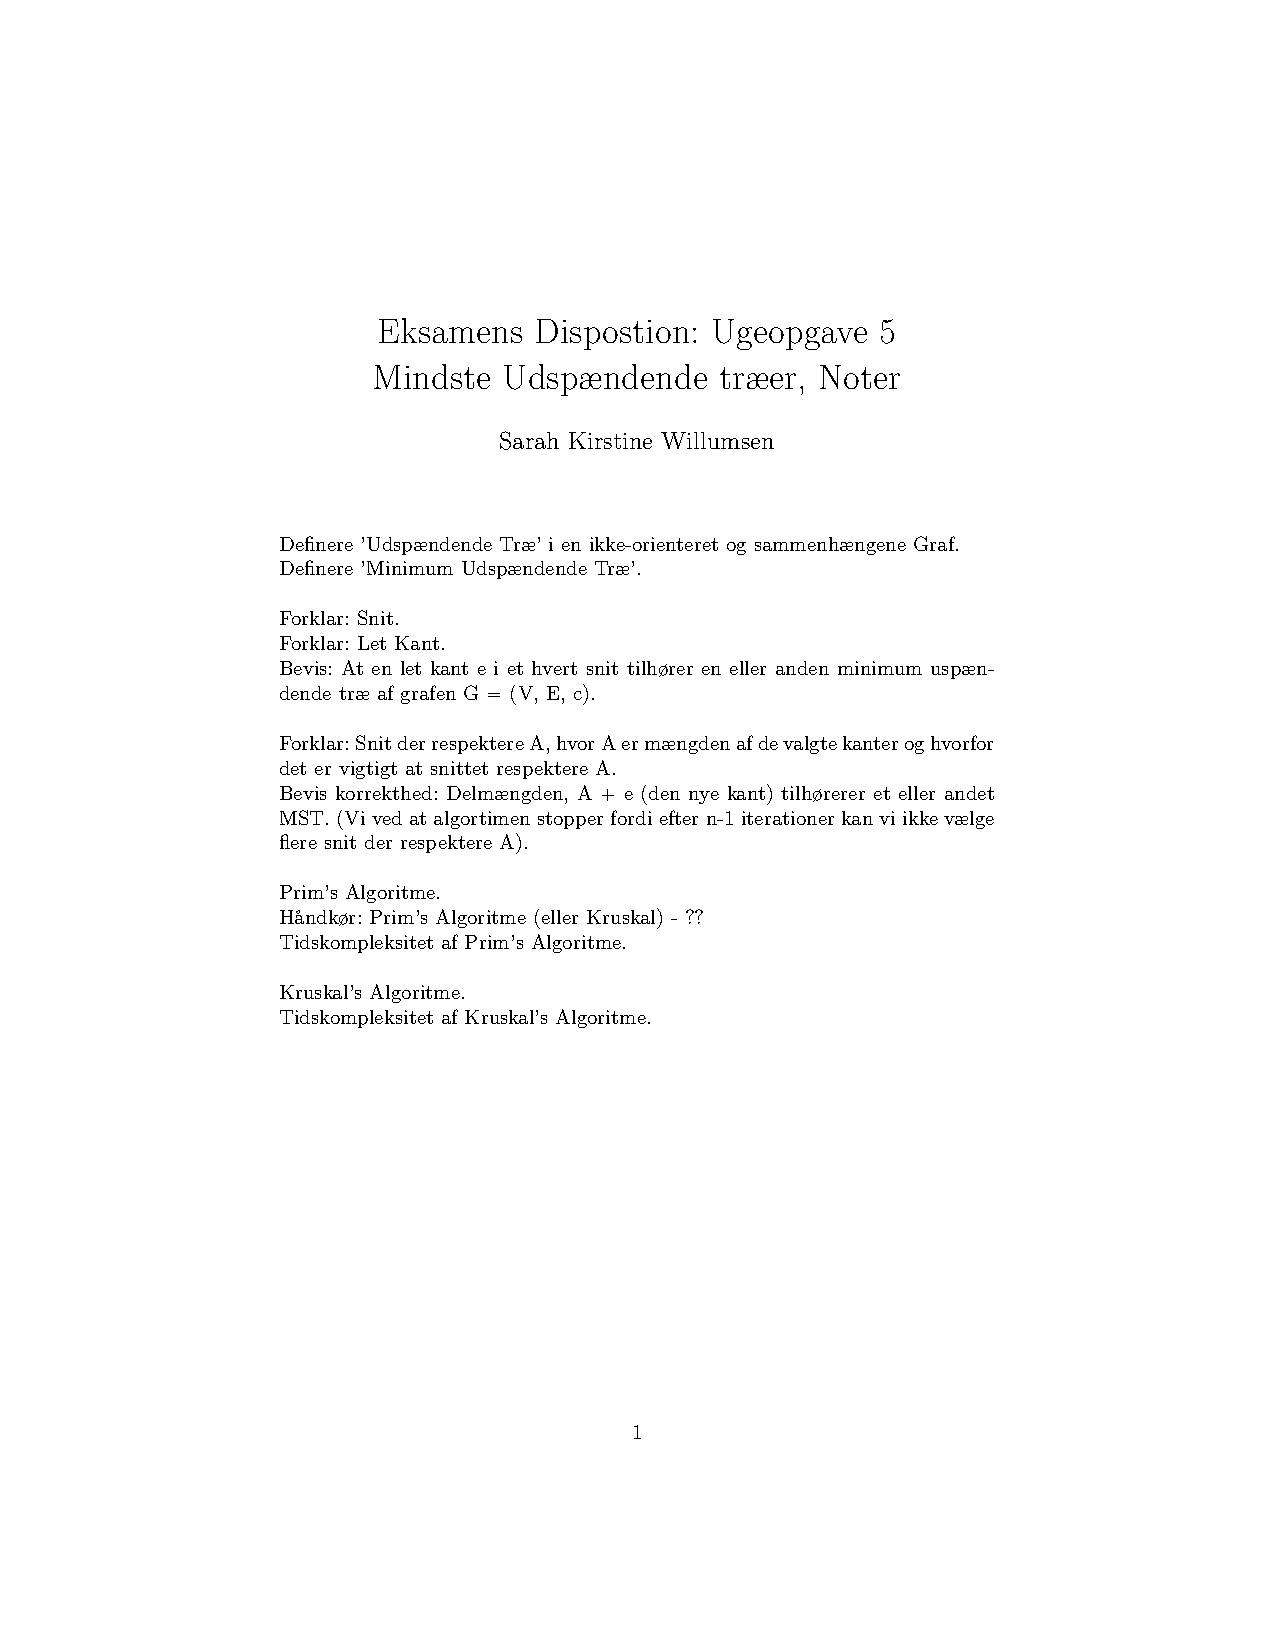
\includepdf[pages=-, offset=-30 50]{Materials/Sarah.pdf}
        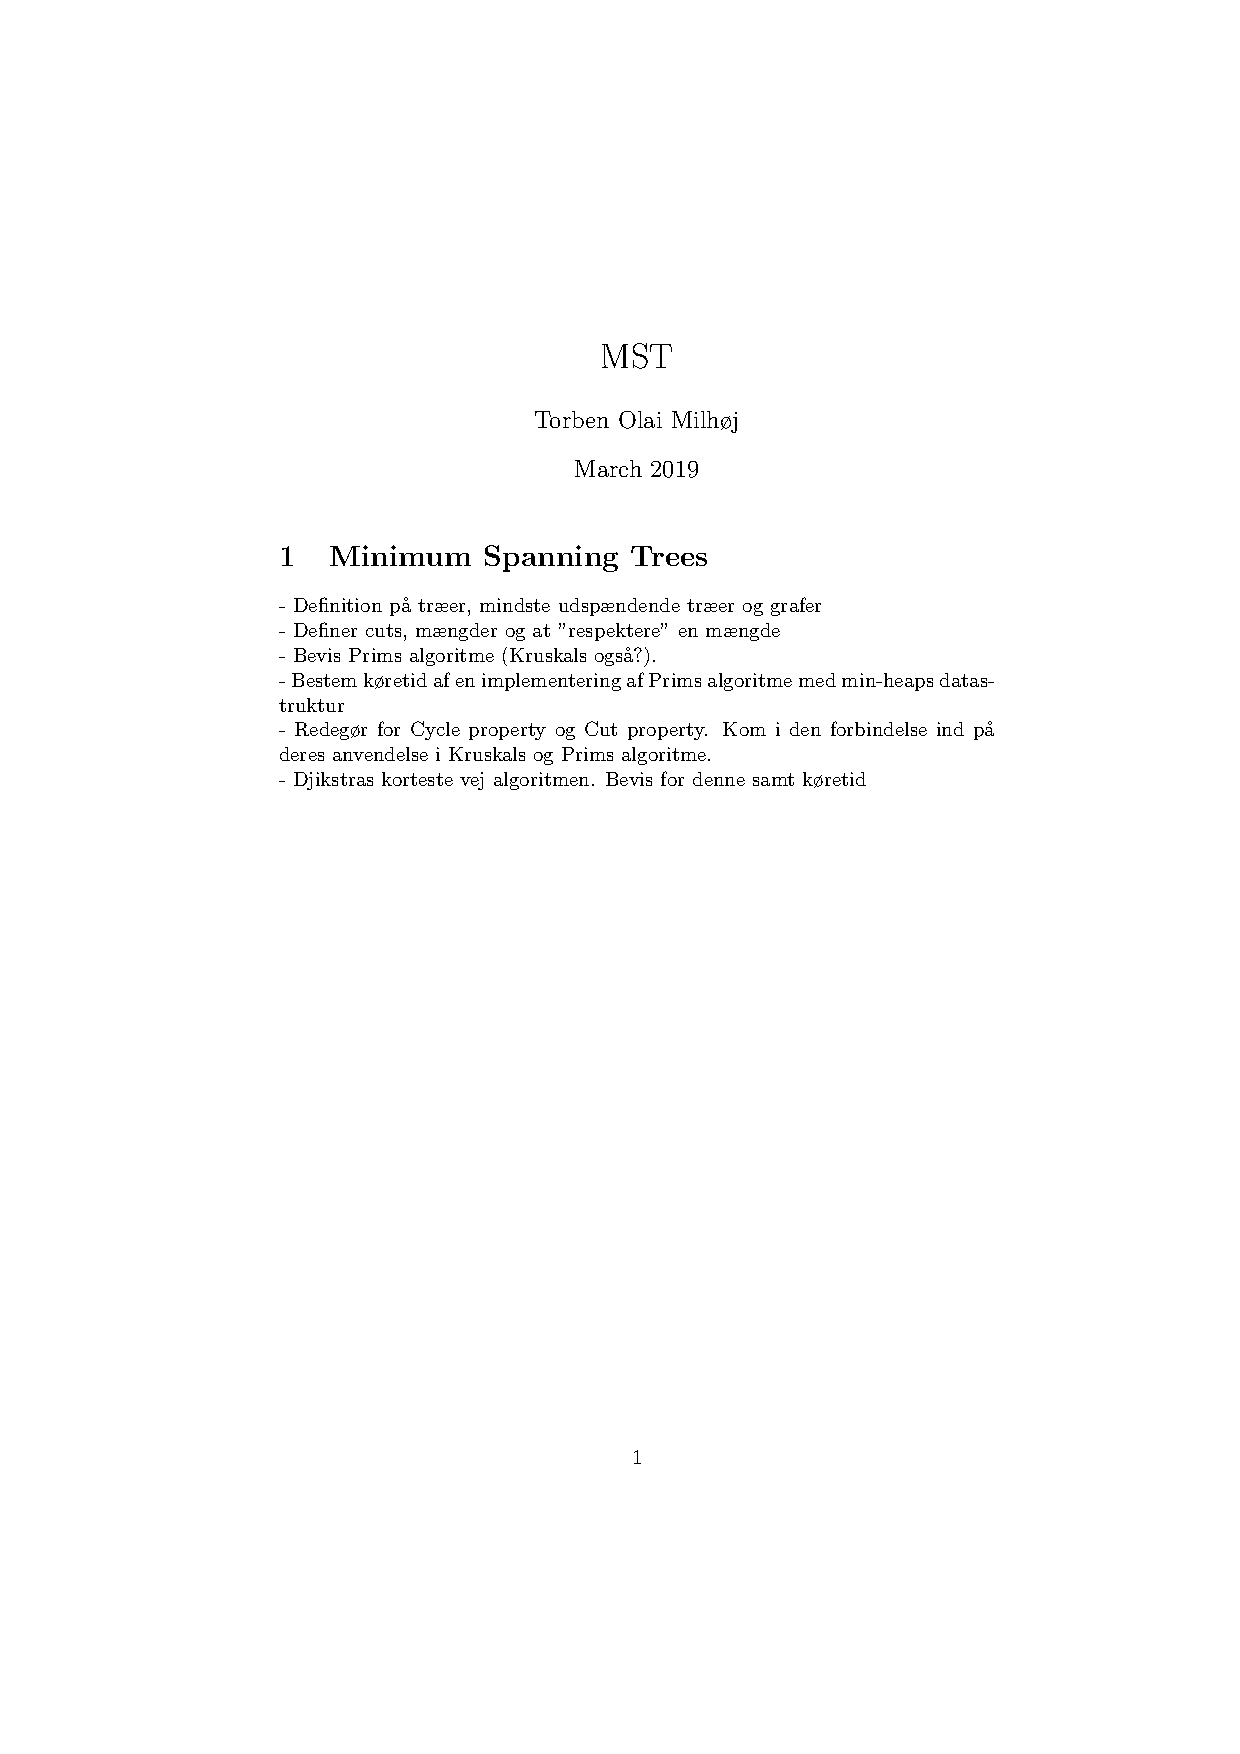
\includepdf[pages=-, offset=-30 50]{Materials/Torben.pdf}
    \end{document}
